%!TEX root = ../thesis.tex

\subsection{Flipping Blue $Z$'s}
\thispagestyle{plain}
\label{ss:flipBlueZ}

  The \rel provided by the sweepcycle algorithm of Section \ref{ss:sweep} often is vertically one-sided but not always. One example is the graph in Figure \fxwarning{TODO give such a graph}
  We prefer to obtain a vertically one-sided \rel since if we then flip edges to break large blue faces we cannot accidentally create many-sided vertical segments. Hence we will in this section modify the current \rel to make it vertically one-sided while maintaining the nice property of Lemma \ref{lm:sweep:NoTwoSplitsAboveEachOther}.


  In the case that this \rel is not one-sided there must be a blue $Z$ (see Figure \ref{fig:zflip:blueZ})

  \begin{figure}[h]
    \centering
    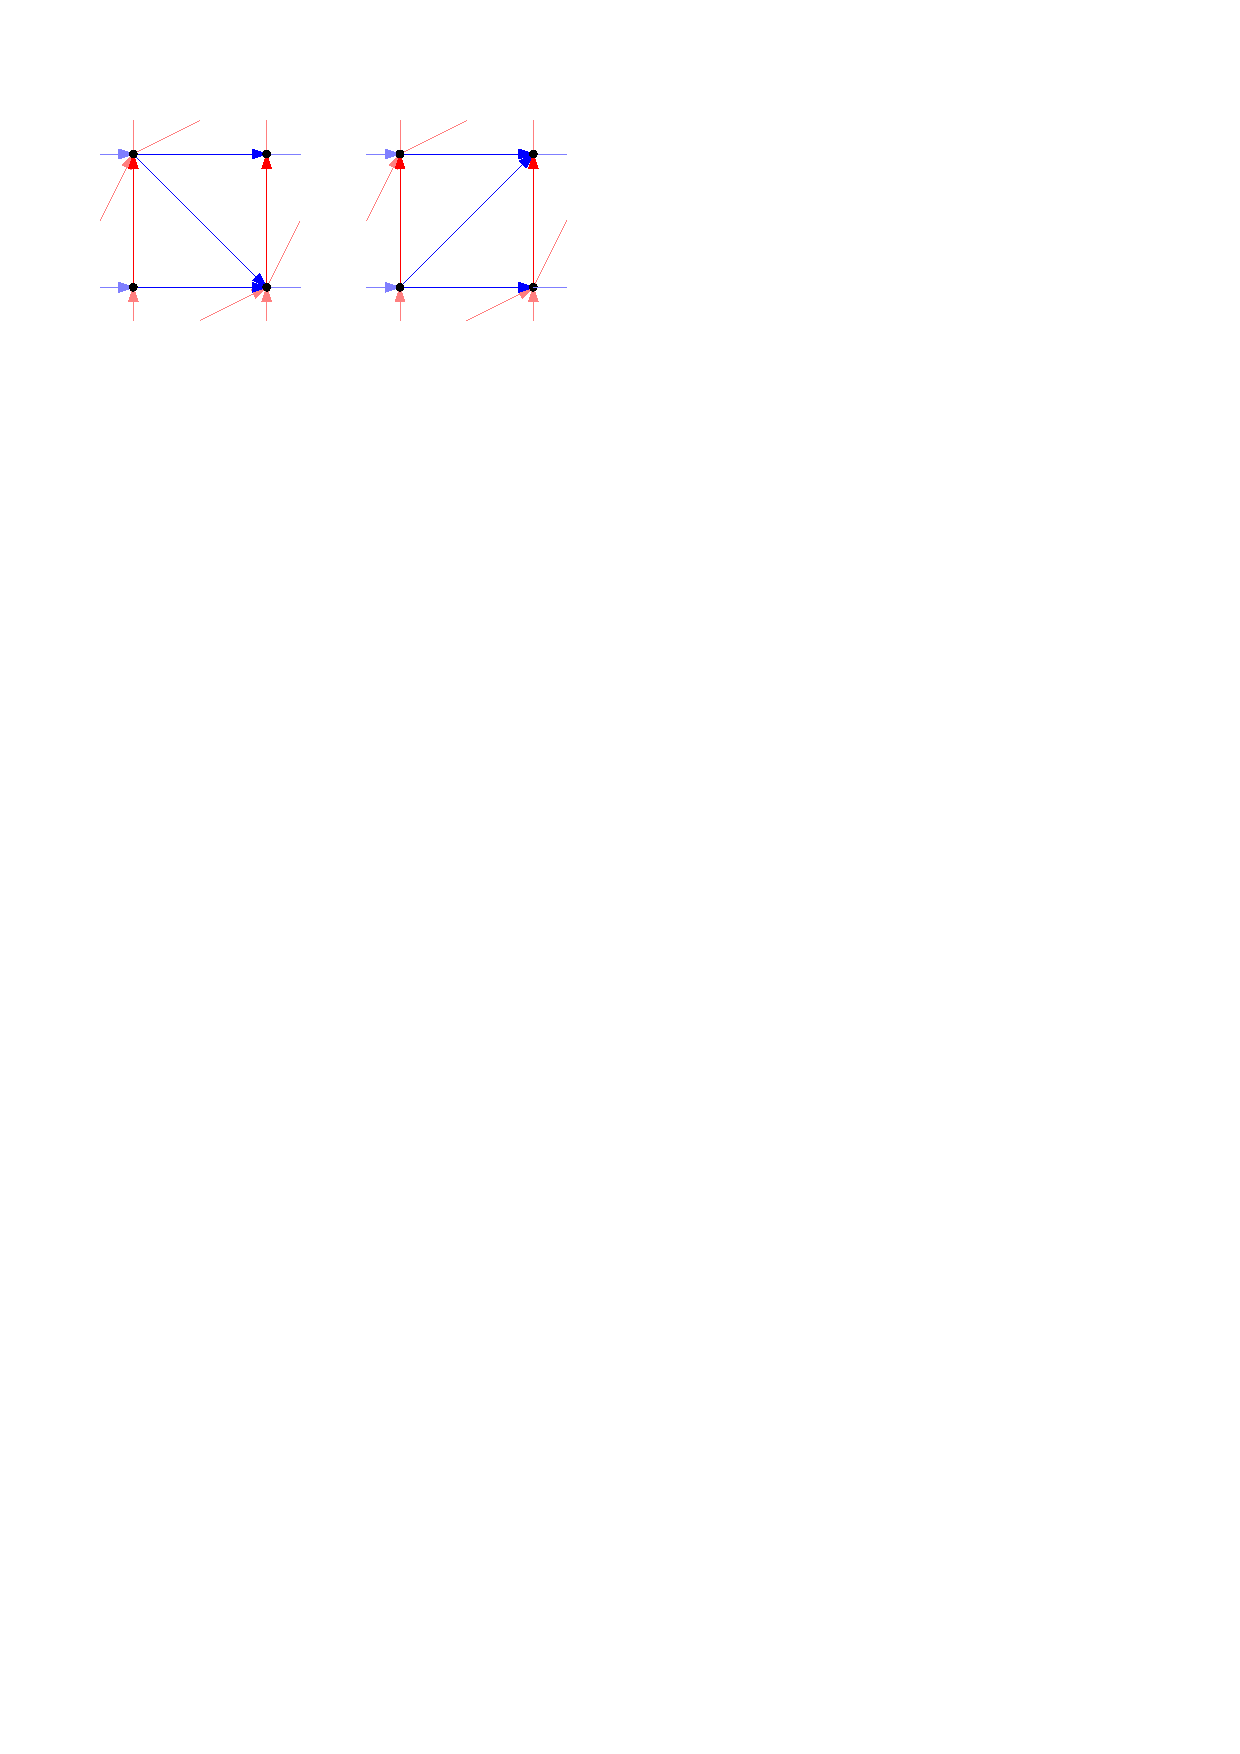
\includegraphics[scale=1]{unifiedAlgo/img/zflip/blueZ.pdf}
    \caption{The two possible blue $Z$'s}
    \label{fig:zflip:blueZ}
  \end{figure}

  We will say that such a $Z$ consists of a \emph{top}, \emph{bottom} and \emph{midlle} edge in straightforward manner. \fxnote{I have some introduction on this subject somewhere}


  As long as the \rel is not vertically one-sided we find such a blue $Z$ and recolor its middle edge as in Figure \ref{fig:zflip:flip}. We will say that this edge is \emph{flipped}

  Note that both flips transfer one valid \rel to another valid \rel. If the interior vertex condition was fulfilled in Figure \ref{fig:zflip:blueZ} then it is also fulfilled in Figure \ref{fig:zflip:flip}.

   We do this until the \rel is vertically one-sided. Since every flip reduces the number of blue edges by one this is a finite procedure.

  \begin{figure}[h]
    \centering
    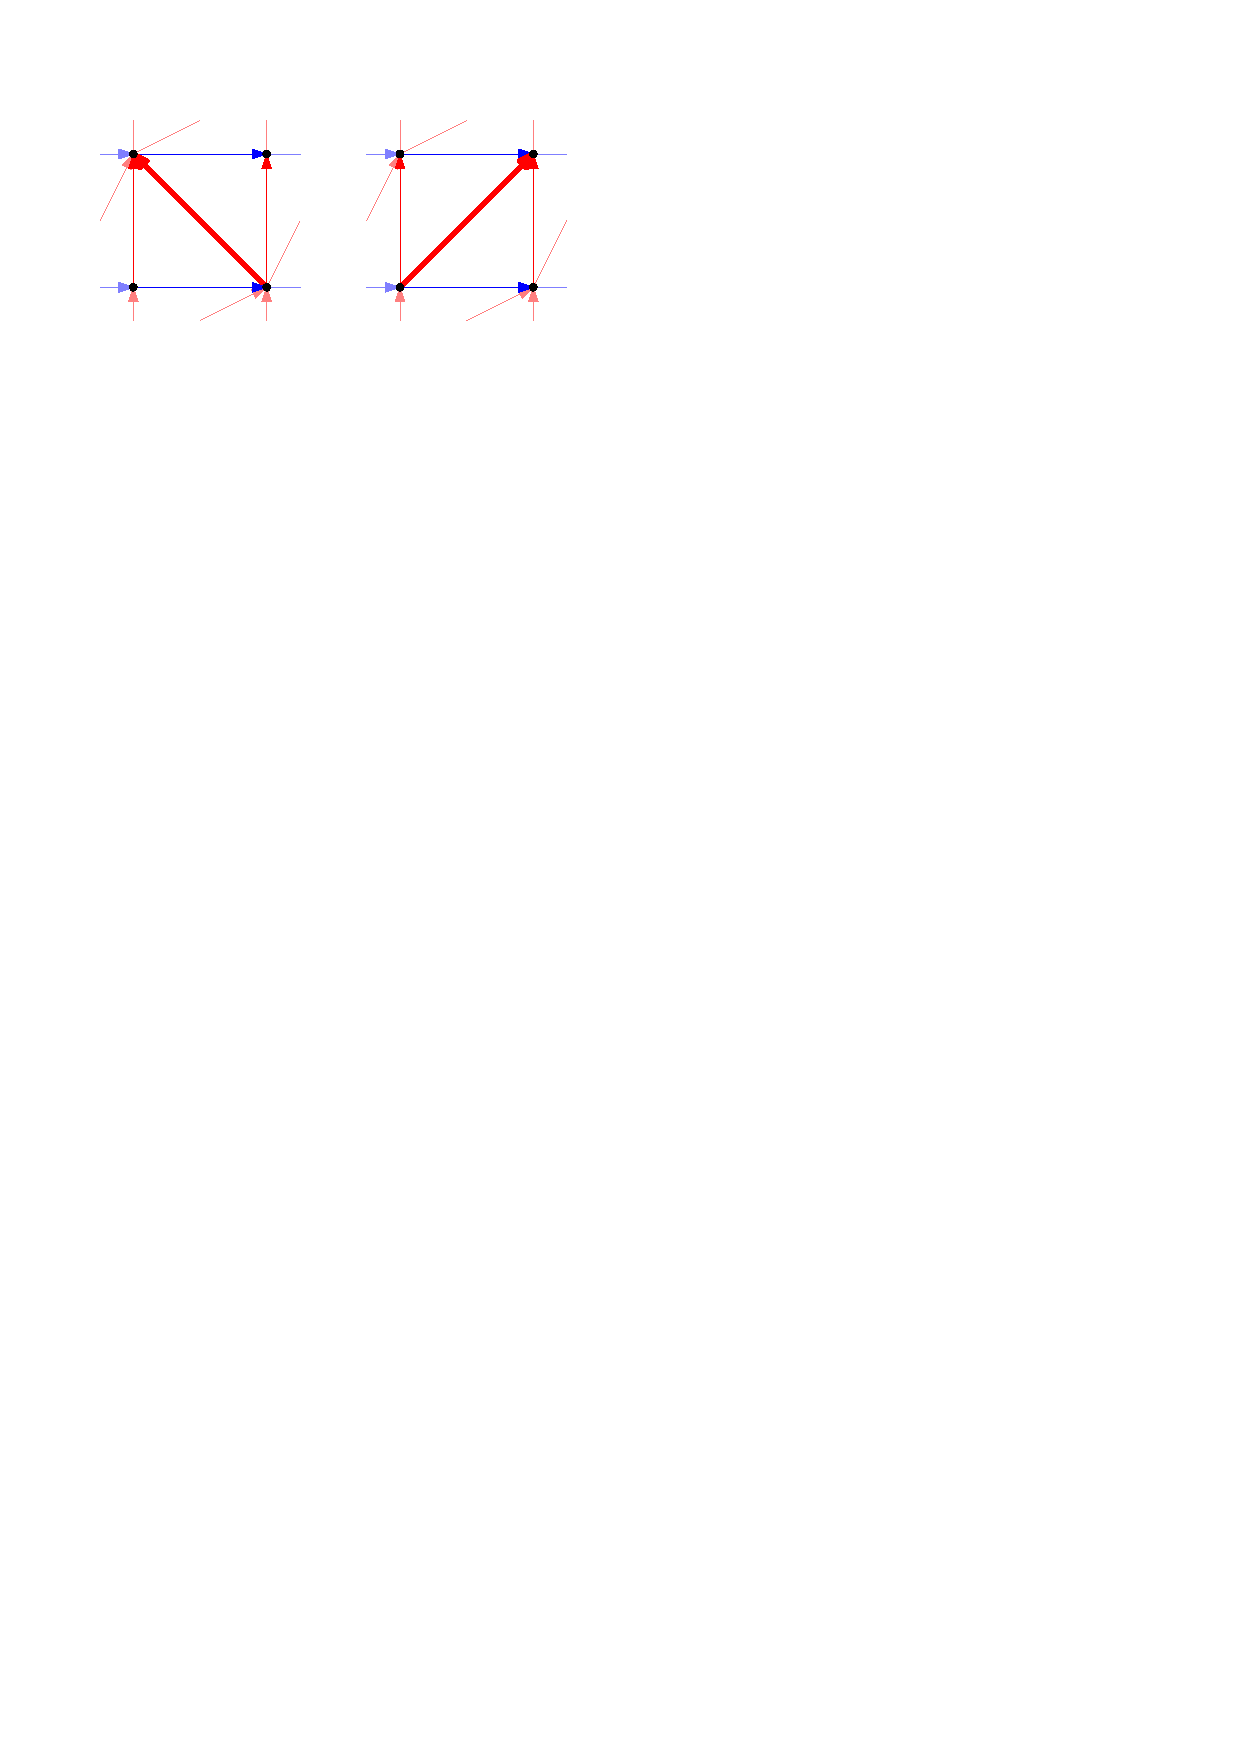
\includegraphics[scale=1]{unifiedAlgo/img/zflip/flip.pdf}
    \caption{The flip}
    \label{fig:zflip:flip}
  \end{figure}

  \begin{lemma}
    \label{lm:sweep:vertOnsided}
    The resulting REL is vertically one-sided
  \end{lemma}
  \begin{proof}
    By construction we flip all blue $Z$'s. If we do not have any more $Z$'s then the remaining \rel is vertically one-sided. \fxnote{refer to some lemma?}
  \end{proof}

  \begin{lemma}
    \label{lm:sweep:NoTwoSplitsAboveEachOtherVertOnesided}
    Lemma \ref{lm:sweep:NoTwoSplitsAboveEachOther} still holds.
    \fxwarning{TODO This must be restated}
  \end{lemma}

  \begin{proof}
    Flipping middle edges of these $Z$'s  can only reduce the number of split vertices.

    For a split vertex $v$ adjacent to $\pS$ we can note that the edge $vw$ will not be flipped because it can not be a middle edge. Hence $w$ is still on the bottom path and still not the handle of a big topfan.

    If $v$ is a split vertex due to a chord let us note the following.
    The edges of $\P$ and $ab$ can not have been flipped since then we would find a monochromatic red triangle while a flip leads to another valid \rel. Hence $w$ is still on the bottom path trough $v$ and still can not be the handle of a large topfan.
  \end{proof}
